%\chapter{On control of harmonic waves in  an acoustic metamaterial}
\chapter{Управление гармоническими волнами в акустическом метаматериале}

%\fixme{Abstract}
  
%\section{Introduction}
\section{Введение}

%In this paper we study numerically generation  of harmonic waves in  a linear metamaterial mass-in-mass model.  The boundary harmonic excitation is shown to produce both the acoustic and optic harmonic waves outside the band gap while no wave propagation is obtained inside the bamd gap. Then the switch-on/off control is developed to see how to change the shape of the harmonic waves inside and outside the band gap.

%Generation of harmonic waves in a mass-in mass model of an acoustic metamaterial is considered. It is shown numerically that outside the band gap, the boundary harmonic excitation gives rise to a formation of periodic waves whose profile gradually coincides with the profile of the exact travelling wave harmonic solution. No waves are generated by the boundary excitation inside the band gap. A switch-on/off control is developed to achieve the formation of the harmonic waves inside the band gap.
В данной главе исследуются вопросы распространения и генерации гармонических волн для модели цепочки <<масса-в-массе>> \cite{Huang2009} акустического метаматериала. Численно показано, что вне запрещенной зоны возбуждение гармоники на границе материала приводит к образованию периодических волн, профиль которых постепенно совпадает с профилем точного гармонического решения в виде бегущей волны. Граничное возбуждение внутри запрещенной зоны не приводит к возникновению волн. С помощью управляющего воздействия вида <<включение-выключение>> достигается формирования гармонических волн внутри запрещенной зоны.

%\fixme{В этой статье} мы численно изучаем генерацию гармонических волн в линейной модели массы к массе метаматериала. Показано, что граничное гармоническое возбуждение создает как акустические, так и оптические гармонические волны за пределами запрещенной зоны, в то время как внутри запрещенной зоны распространения волн не происходит. \fixme{Затем разрабатывается управление switch-on/off, чтобы увидеть, как изменить форму гармонических волн внутри и за пределами запрещенной зоны}.

%\section{Statement of problem}
\section{Постановка задачи}

%\fixme{Нужно поправить перевод}

%Consider a  chain   when interaction between the  masses,  $m$,  is modeled by linearly- elastic springs \cite{Huang2010}. An elastic internal oscillator is modelled by the additional masses $m_1$ , attached by springs to each mass $m$ in the chain, and this interaction is also linear and elastic. Masses $m_1$ do not interact directly between themselves. The displacement of the mass $m$ with the number $n$ is denoted by $x_n$, while that of $m_1$ is denoted by $y_n$.
Рассмотрим цепочку, в которой взаимодействие между массами $ m $ моделируется линейно-упругими пружинами \cite {Huang2009, Huang2010}. Упругий внутренний осциллятор моделируется дополнительными массами $ m_1 $, прикрепленными пружинами к каждой массе $ m $ в цепочке, и это взаимодействие также является линейным и упругим. Массы $ m_1 $ не взаимодействуют между собой напрямую. Смещение массы $ m $ с числом $ n $ обозначено $ x_n $, а перемещение $ m_1 $ --- $ y_n $. \fixme{Здесь нужен рисунок.}

\begin{equation}
\ddot{x_n}=\beta_0 (x_{n-1}-2x_n+x_{n+1})+\eta \beta_1 (y_n-x_n), 
\label{eq1}
\end{equation}
\begin{equation}
\ddot{y_n}=-\beta_1 (y_n-x_n). \label{eq2}
\end{equation}
%Here $\eta=m_1/m$, while the linear stiffness of the spring of the chain is $\beta_0 m$,  the nonlinear stiffness is $\beta_3 m$. Corresponding linear and nonlinear stiffnesses of the attached spring are $\beta_1 m_1$ , $\beta_2 m_1$ respectively.
Здесь $ \eta = m_1 / m $, линейная жесткость пружины цепочки --- $ \beta_0 m $, соответствующая линейная жесткость прикрепленной пружины равна $ \beta_1 m_1 $. 
\begin{figure*}[h]
\begin{center}
%\begin{flushleft}
%\end{flushleft}
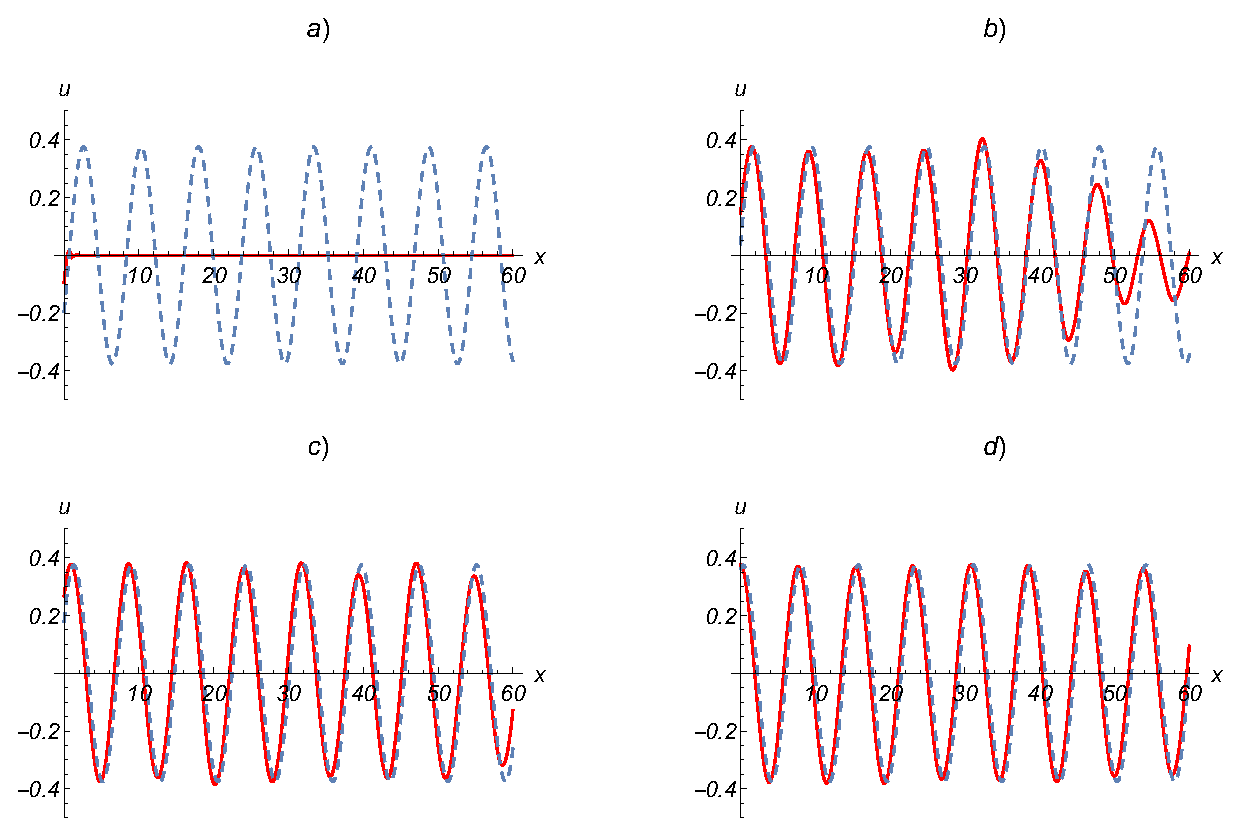
\includegraphics[width=1.0\textwidth]{new_pic/fig1.eps}
\end{center}
%\caption{ Evolution of $u$ wave below the band gap, $\omega<\sqrt{\beta_1}$. Shown by dashed line is the imagine part of the  exact solution (\ref{solfin}) with the frequency $\omega=\omega_a$.  a)$t=0$; b)$ t=t_N/4$; c) $t=t_N/2$, d)$t=t_N$.}
\caption{ Эволюция волны $ u $ ниже запрещенной зоны, $\omega<\sqrt{\beta_1}$. Пунктирной линией обозначена мнимая часть точного решения (\ref{solfin}) с частотой $\omega=\omega_a$.  a)$t=0$; b)$ t=t_N/4$; c) $t=t_N/2$, d)$t=t_N$.}
\label{fg1}
  \end{figure*}
%We proceed with a continuum limit of Eqs. (\ref{eq1}), (\ref{eq2}). Following the standard procedure we introduce the continuum functions $u(x,t)$, $v(x,t)$ for description of the displacements of the masses $m$, $m_1$ with the number $n$ while the continuum displacements of the neighboring masses are sought using the Taylor series around $u$. Retaining only the first nonzero term in the expansion we obtain
Перейдем к континуальному пределу уравнений (\ref {eq1}), (\ref {eq2}). Следуя стандартной процедуре, введем функции континуума $ u(x, t) $, $ v(x, t) $ для описания перемещений масс $ m $, $ m_1 $ с числом $ n $, а континуальные значения смещений соседних масс ищутся с помощью разложения в ряд Тейлора относительно $ u $. Оставляя в разложении только первый ненулевой член, получаем
\begin{equation}
u_{tt}=\beta_0 h^2 u_{xx}+\eta \beta_1 (v-u), \label{eq3}
\end{equation}
\begin{equation}
v_{tt}=-\beta_1 (v-u), \label{eq4}
\end{equation}
%where $h$ is a distance between the masses $m$ in the chain.
где $ h $ --- расстояние между массами $ m $ в цепочке.
%The conventional traveling wave solution is sought as
Классическое решение в виде бегущей волны ищется как
\begin{equation}\label{sol}
 u=A\exp (\imath(p~ x - \omega~ t- p~ x_0)), ~
   v=B \exp (\imath(p~ x - \omega~ t-p~ x_0))
\end{equation}
%Substituting Eq. (\ref{sol}) into Eqs. (\ref{eq3}), (\ref{eq4}) one obtains the known dispersion relation \cite{Huang2010}
Подставляя уравнение (\ref{sol}) в уравнения (\ref{eq3}), (\ref{eq4}) получаем известное дисперсионное соотношение \cite{Huang2009,Huang2010}
\[
\omega^4 -(\beta_1(1+\eta)+\beta_0 p^2 h^2)\omega^2+\beta_0 \beta_1 p^2 h^2=0.
\]
%whose solution is
чье решение суть 
\begin{equation}\label{acdiscr}
\omega_a^2=\frac{\beta_1(1+\eta)+\beta_0 h^2 p^2}{2}-\frac{\sqrt{D}}{2},
\end{equation}
\begin{equation}\label{optdiscr}
\omega_o^2=\frac{\beta_1(1+\eta)+\beta_0 h^2 p^2}{2}+\frac{\sqrt{D}}{2},
\end{equation}
%where
где
\[
D=(\beta_1(1+\eta)+\beta_0 h^2 p^2)^2-4\beta_0 h^2 p^2,
\]

%Also the expression for $A$ through  $B$ is obtained giving rise to the solution for $u$ and $v$ in the final form
Таким же образом можно выразить $A$ через $B$, что дает решение для $u$ и $v$ в окончательном виде
\begin{equation}\label{solfin}
 u=\frac{\beta_1-\omega^2}{\beta_1}~B\exp (\imath(p~ x - \omega~ t- p~ x_0)), ~
   v=B \exp (\imath(p~ x - \omega~ t- p~ x_0)),
\end{equation}
%where the frequency is  $\omega=\omega_a$,  or $\omega=\omega_o$, $x_0$ accounts for an initial phase.
где частота равна $ \omega = \omega_a $ или $ \omega = \omega_o $, $ x_0 $ учитывает начальную фазу.
%The acoustic band frequency varies from $0$ to $\sqrt{\beta_1}$\, while the optic one lies in the interval $(\sqrt{\beta_1(1+\eta)}, \infty)$. Therefore, there is a band gap $\sqrt{\beta_1}<\omega<\sqrt{\beta_1(1+\eta)}$ where no harmonic traveling wave propagates.
Акустическая ветвь лежит в диапазоне частот от $ 0 $ до $ \sqrt {\beta_1} $, а оптическая --- в интервале $(\sqrt{\beta_1(1+\eta)}, \infty)$. Следовательно, существует запрещенная зона $ \sqrt {\beta_1} <\omega <\sqrt {\beta_1 (1+ \eta)} $, где бегущие гармонические волны не могут распространяться.

%\section{Generation of harmonic waves}
\section {Возбуждение гармонических волн}
%The analysis in the previous Section is based on the particular traveling wave solution which requires specific initial and boundary conditions for its realization. However, experimental generation of the waves in a metamaterial uses the boundary excitation of the waves. In particular, the following  initial and boundary conditions for $u$ can be employed,
Анализ в предыдущем разделе основан на конкретном решении в виде бегущей волны, которое требует определенных начальных и граничных условий. Однако экспериментальная генерация волн в метаматериале реализуется с помощью возбуждения на границе. В частности, можно использовать следующие начальные и граничные условия для $u$:
\begin{equation}\label{bcu}
u(0,t)=\frac{\beta_1-\omega^2}{\beta_1}~B~ {\text{sin}} (\omega ~t),~u(x,0)=0, ~u(x,0)_t=0,
\end{equation}
%while for $v$ we assume that
а для $ v $ мы предполагаем, что
\begin{equation}\label{bcv}
v(0,t)=B ~{\text{sin}} (\omega ~t),~v(x,0)=0, ~v(x,0)_t=0.
\end{equation}
%This problem can be solved numerically. The Wolfram Mathematica NDSolve command is used to solve Eqs. (\ref{eq3}), (\ref{eq4}) with the conditions (\ref{bcu}), (\ref{bcv}).
Эта задача может быть решена численно. При помощи команды Wolfram Mathematica NDSolve, предназначенной для численного решения дифференциальных уравнений в частных производных, будет решаться система уравнений (\ref {eq3}), (\ref{eq4}) с условиями (\ref {bcu}), (\ref {bcv}).
%%%The interval of calculations is $0<x<x_N$,
%The interval of interest is $0<x<x_N$, the absorbing boundary conditions are imposed at $x=x_N$ using the following masking technique. The calculation domain $0 < x < 3 x_N$ is being splitted into two parts:  $0 < x < x_N$ and  $x_N < x < 3 x_N$ while the system of Eq. (\ref{eq1}), (\ref{eq2}) is replaced with
Будем считать, что интервал интереса --- $ 0 <x < x_N $ (в котором будут качественно исследоваться свойства решений), а в точке $ x = x_N $ накладываются поглощающие граничные условия с использованием следующей техники. Расчетная область $ 0 <x < 3 x_N $ делится на две части: $ 0 <x <x_N $ и $ x_N <x <3 x_N $, в то время как система уравнений (\ref {eq1}), (\ref {eq2}) заменяется на следующую,
$$
U_{t}=\beta_0 h^2 u_{xx}+\eta \beta_1 (v-u)
$$
$$
u_{t}=U + u f_{\text{mask}},
$$
$$
v_{tt}=-\beta_1 (v-u),
$$
%where $f_{\text{mask}} = \log \left(\tanh{0.03 (3 x_N - x)}\right)^2$. By this way, as far as $f_{\text{mask}}$ is effectievely zero in the interval of interest the exact system of Eq.  (\ref{eq1}), (\ref{eq2}) is being solved there. While for the rest part of the domain $f_{\text{mask}}$ is negative and decreasing with $x$,4 which leads to the corresponding decrease of the amplitude of the each wave frequency traveling through. The resulting amplitude of wave at $x = 3 x_N$ becames numerically very close to zero leading to nothing be reflected to the interval of interest from the $x = 3 x_N$ boundary.
где $ f_{\text {mask}} = \log \left(\tanh {0.03 (3 x_N - x)} \right) ^ 2 $. Таким образом, поскольку $ f_{\text{mask}} $ фактически равна нулю в интервале интереса, внутри него решается в точности система (\ref{eq1}), (\ref{eq2}). В то время как для остальной части области $ f_{\text{mask}} $ отрицательна и уменьшается с $ x $, что приводит к соответствующему уменьшению амплитуды со временем всех гармоник, пробегающих в этом интервале. Результирующая амплитуда волны при $ x = 3 x_N $ численно становится очень близкой к нулю, что приводит к тому, что отражением от границы $ x = 3 x_N $ на интервал интереса можно пренебречь. Данный подход по сути разделяет расчетную область на две части, в одной из которых представляет собой нефизичный поглощающий слой. Следует отметить, что существуют и другие методы задания поглощающих граничных условий, в том числе и не требующие при этом расширения интервала и увеличения вычислительных затрат \cite{clayton1977absorbing, cerjan1985nonreflecting, berenger1994perfectly, renaut1996pseudospectral}. Отсутствие такого слоя требует задание специального граничного условия в поглощающей точке в виде уравнения, допускающего распространение гармонических волн только в одном направлении и обладающего максимально совпадающим с основным уравнением дисперсионным соотношением для этого направления \cite{halpern1988wide, lindman1975free}. Получение такого приближенного уравнения и соответствующей численной схемы в данном случае не были реализованы, так как простые численные эксперименты показали, что предложенная техника обладает достаточной точностью и скоростью работы для необходимых исследований.
\begin{figure*}
\begin{center}
%\begin{flushleft}
%\end{flushleft}
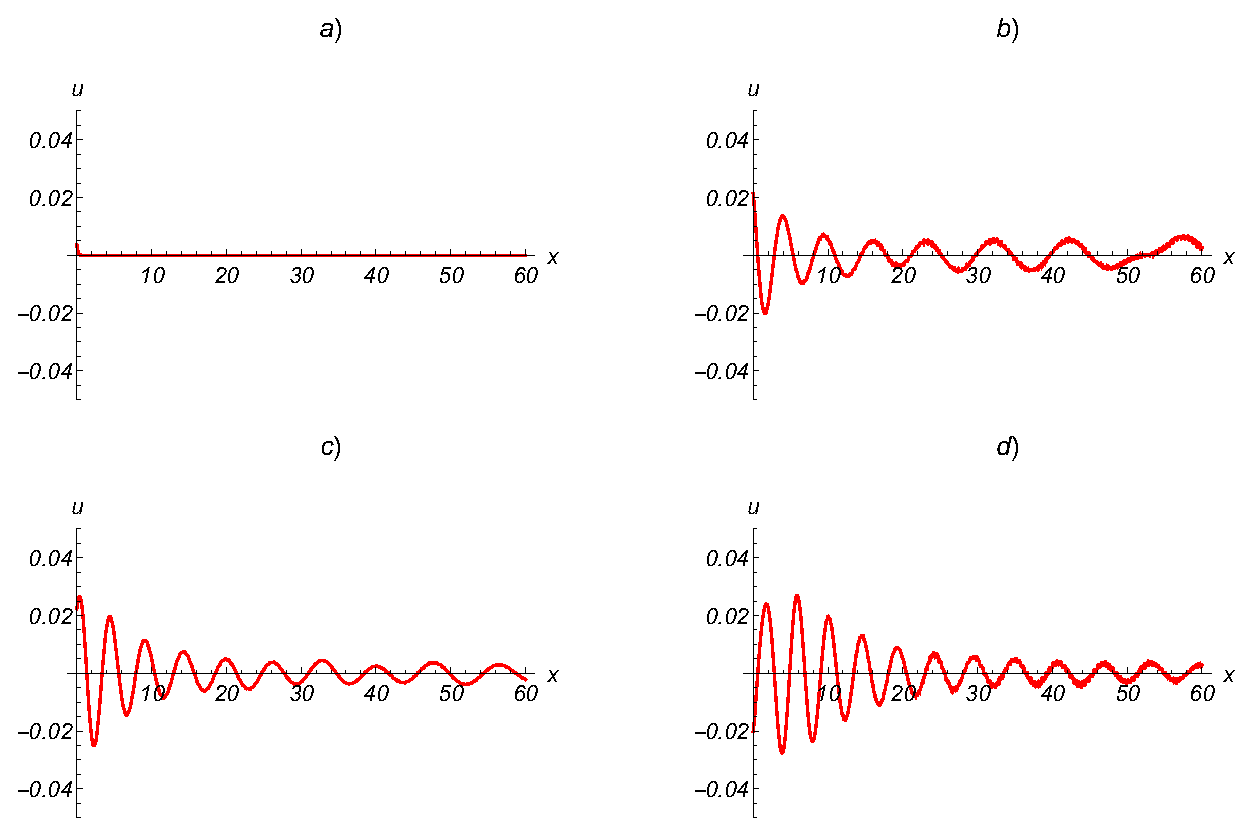
\includegraphics[width=1.0\textwidth]{new_pic/fig2.eps}
%\caption{ Evolution of $u$ wave at the lower boundary of the band gap, $\omega \approx \sqrt{\beta_1}$,  $\omega=0.3$.  a)$t=0$; b)$ t=t_N/4$; c) $t=t_N/2$, d)$t=t_N$.}
\caption{Эволюция волны $ u $ на нижней границе запрещенной зоны, $ \omega \approx \sqrt {\beta_1} $, $\omega = 0.3$. а) $ t = 0 $; б) $ t = t_N / 4 $; в) $ t = t_N / 2 $, г) $ t = t_N $.}
\label{fg2}
\end{center}
\end{figure*}

  
%The aim of calculations is to see how the harmonic boundary excitation gives rise to the harmonic wave  in time.  The imaginary parts of the solutions (\ref{solfin}) will be compared with the numerical results. For this purpose the initial position $x_0$  in Eqs. (\ref{solfin}) will be chosen so as to coincide as close as possible the numerical and analytical curves at the final time of calculations, $t=t_N$. Then both curves are placed together for the preceding moments of times. Also, the realization of the band gap will be studied by varying the frequency $\omega$ ib the boundary conditions (\ref{bcu}), (\ref{bcv}) from zero through the band gap. Therefore the values of frequency $\omega$ is defined while the wave number of the exact solution, $p$, is calculated through it using the dispersion relation,
Цель расчетов --- увидеть, как гармоническое возбуждение на границе порождает гармоническую волну во времени. Мнимые части решений (\ref{solfin}) будут сравниваться с численными результатами. Для этого относительное положение точки $ x_0 $ в уравнениях (\ref{solfin}) будет выбрана таким образом, чтобы как можно ближе совпадали численные и аналитические кривые в последний момент вычислений, $ t = t_N $. Для иллюстрации результатов обе кривые помещаются в соответствующее положения для предыдущих моментов времени. Кроме того, влияние запрещенной зоны будет изучаться путем увеличением частоты $ \omega $ в граничных условиях (\ref{bcu}), (\ref{bcv}) от нуля и далее через запрещенную зону. Волновое число точного решения $ p $ вычисляется по значению  $ \omega $ него с использованием дисперсионного соотношения,
\[
p=\omega\sqrt{\frac{\beta_1(1+\eta)-\omega^2}{\beta_0 h^2(\beta_1-\omega^2)}}.
\]
%The values of the coefficients are chosen as $t_N = 600; x_N = 60;\beta_0=1, h = 0.5; \beta_1 = 0.1; \eta = 0.5;  B=0.25$. Then the band gap is $0.316<\omega<0.387$.
Значения коэффициентов выбраны следующими, $t_N = 600; x_N = 60;\beta_0=1, h = 0.5; \beta_1 = 0.1; \eta = 0.5;  B=0.25$, что соответствует запрещенной зоне $0.316<\omega<0.387$.
  
%Shown in Fig \ref{fg1} is the formation of harmonic wave $u$ at various times when the excitation frequency lies below the band gap, $\omega<\sqrt{\beta_1}$, $\omega=0.2$, $x_0= 15.8$. The exact solution is placed on each time sketch a)-d).  One can see that initially undisturbed stage a) transforms to a non-harmonic wave which partially coincides with the harmonic exact traveling wave solution at the stage b). The last two stages c) and d) demonstrate almost full similarity between numerical and analytical solution.
На рисунке \ref{fg1} показано формирование гармонической волны $ u $ в разные моменты времени, когда частота возбуждения лежит ниже запрещенной зоны, $ \omega <\sqrt {\beta_1} $, $ \omega = 0.2 $, $ x_0 = 15.8 $. Численное решение и точная гармоническая волна с учетом относительного смещения $x_0$ представлены на графиках a) - d). Видно, что изначально невозмущенная стадия а) трансформируется в негармоническую волну, которая частично совпадает с гармоническим точным решением бегущей волны на стадии b). Последние два этапа c) и d) демонстрируют почти полное сходство численного и аналитического решений.
\begin{figure*}
\begin{center}
%\begin{flushleft}
%\end{flushleft}
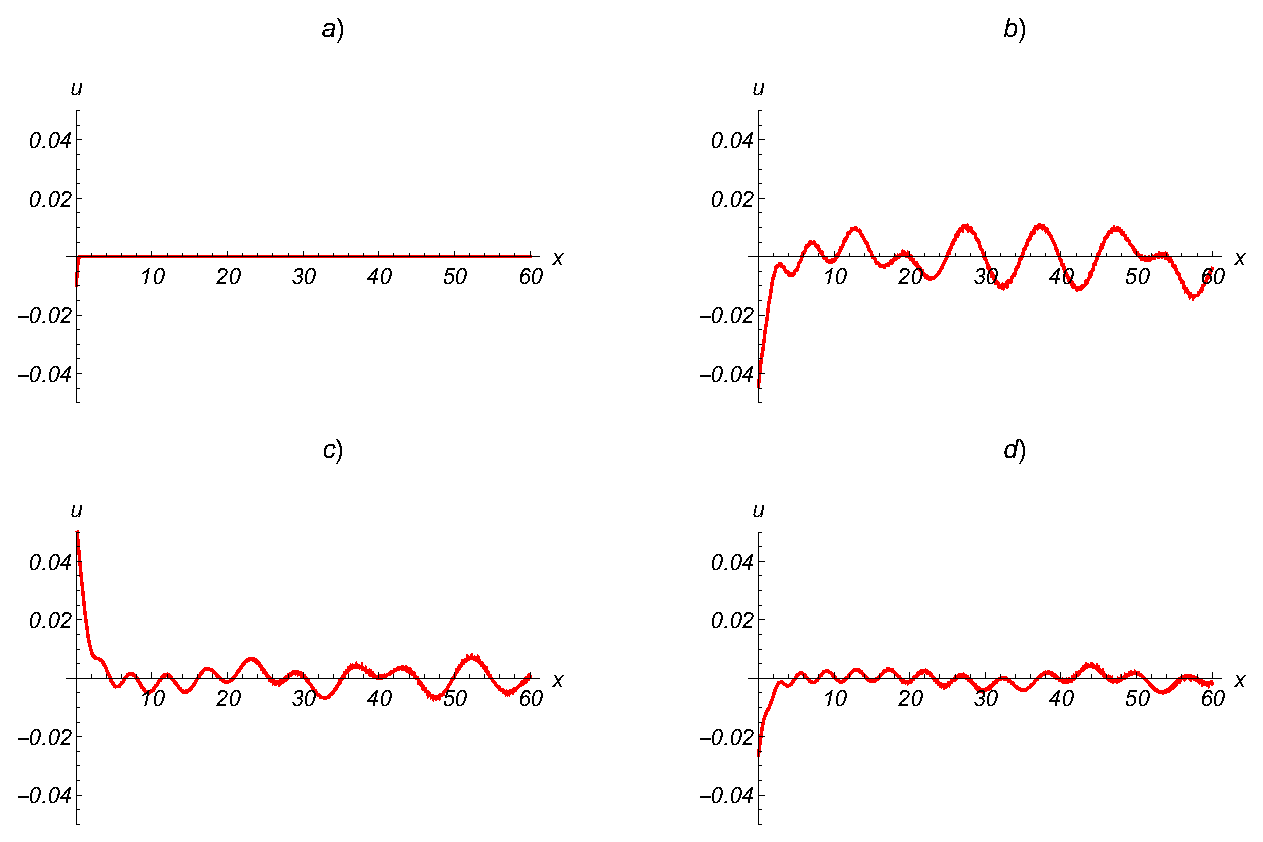
\includegraphics[width=1.0\textwidth]{new_pic/fig3.eps}
\end{center}
%\caption{Supression  of $u$ wave inside the band gap, $\sqrt{\beta_1}<\omega<\sqrt{\beta_1(1+\eta)}$, $\omega=0.35$. a)$t=0$; b)$ t=t_N/4$; c) $t=t_N/2$, d)$t=t_N$.}
\caption{Подавление $ u $ волны внутри запрещенной зоны, $\sqrt{\beta_1}<\omega<\sqrt{\beta_1(1+\eta)}$, $\omega=0.35$. a)$t=0$; b)$ t=t_N/4$; c) $t=t_N/2$, d)$t=t_N$.}
\label{fg3}
\end{figure*}
  
%An increase in the excitation frequency up to  the lower boundary of the band gap, $\omega \approx \sqrt{\beta_1}$,  $\omega=0.3$,  results in the formation of the wave shown in Fig. \ref{fg2}. One can see no harmonic wave generation, the amplitude of the wave decays away from the left boundary. The last two stages c) and d) demonstrate almost stable wave dynamics.
Увеличение частоты возбуждения до нижней границы запрещенной зоны $ \omega \approx \sqrt {\beta_1} $, $\omega = 0.3 $ приводит к формированию волны, показанной на Рис. \ref{fg2}. Генерации гармонической волны не наблюдается, амплитуда волны спадает при удалении от левой границы. Последние два этапа c) и d) демонстрируют практически стабильную волновую динамику.
\begin{figure*}
\begin{center}
%\begin{flushleft}
%\end{flushleft}
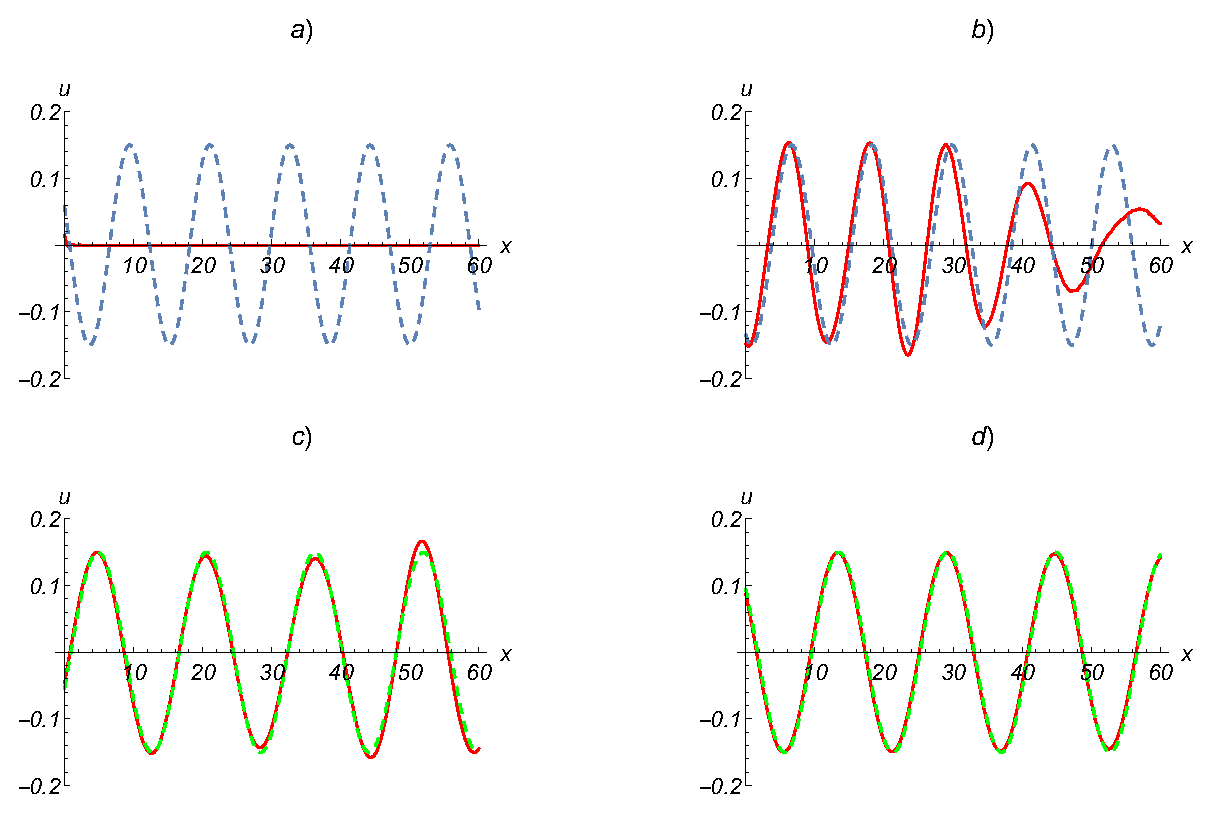
\includegraphics[width=1.0\textwidth]{new_pic/fig4.eps}
\end{center}
%\caption{ Control of evolution of $u$ wave below the band gap, $\omega<\sqrt{\beta_1}$ when the control switches-on at $t=t_N/4$.   a)$t=0$; b)$ t=t_N/4$. Shown by dashed line is the imagine part of the  exact solution (\ref{solfin}) ; c) $t=t_N/2$, d)$t=t_N$. Shown by dashed line is the imagine part of the  exact solution (\ref{solwave}) }
\caption{ Управление эволюцией волны $ u $ ниже запрещенной зоны, $\omega<\sqrt{\beta_1}$ при включении управления в момент $t=t_N/4$. a)$t=0$; b)$ t=t_N/4$. Пунктирной линией обозначена мнимая часть точного решения (\ref{solfin}); c) $t=t_N/2$, d)$t=t_N$. Пунктирной линией показана мнимая часть точного решения (\ref{solwave}) }
\label{fg4}
  \end{figure*}
\begin{figure*}
\begin{center}
%\begin{flushleft}
%\end{flushleft}
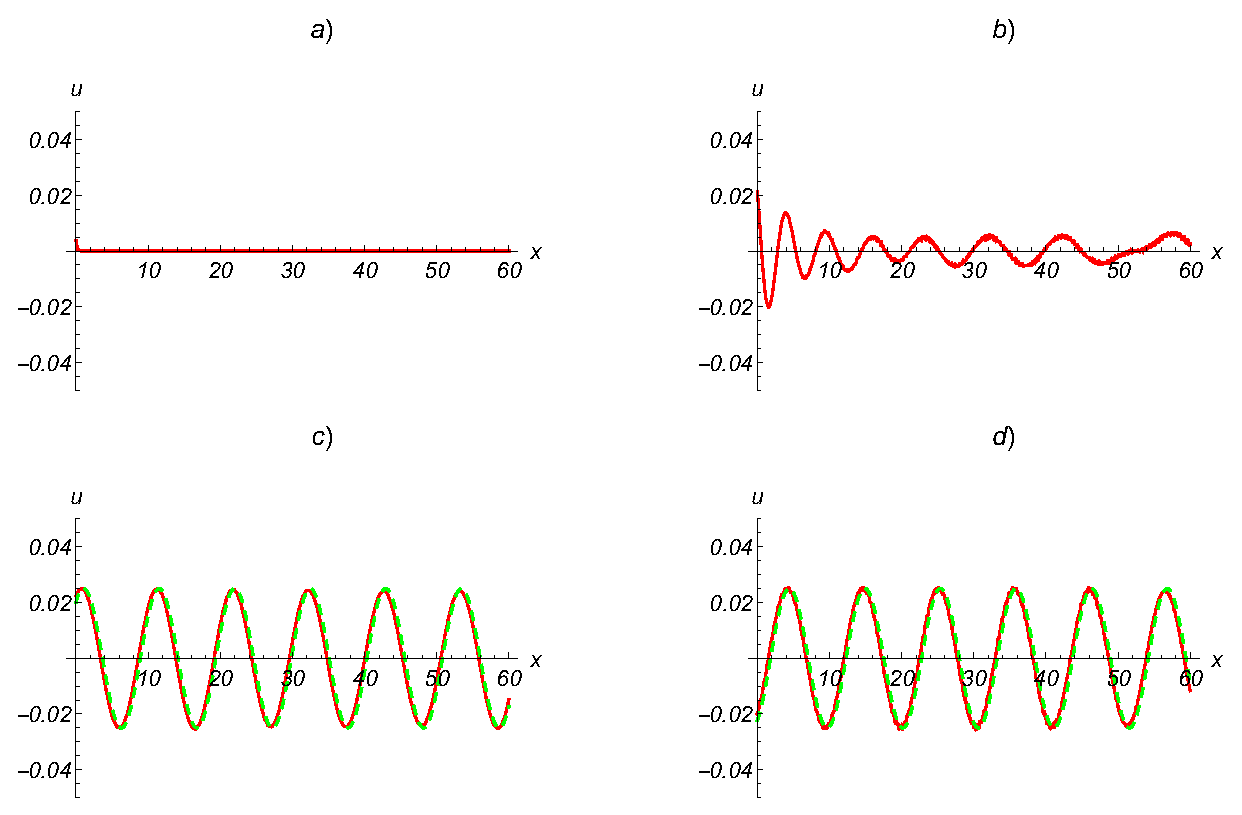
\includegraphics[width=1.0\textwidth]{new_pic/fig5.eps}
\end{center}
%\caption{Control of evolution of $u$ wave at the lower boundary of the band gap, $\omega \approx \sqrt{\beta_1}$, $\omega=0.3$,  when the control switches-on at $t=t_N/4$.   a)$t=0$; b)$ t=t_N/4$ ; c) $t=t_N/2$; d)$t=t_N$. Shown by dashed line in the last two stages  is the imagine part of the  exact solution (\ref{solwave}) .}
\caption{Управление эволюцией $ u $ волны на нижней границе запрещенной зоны, $\omega \approx \sqrt{\beta_1}$, $\omega=0.3$, при включении управления в момент $t=t_N/4$. a)$t=0$; b)$ t=t_N/4$ ; c) $t=t_N/2$; d)$t=t_N$. Пунктирной линией на последних рисунках обозначена мнимая часть точного решения (\ref{solwave}).}
\label{fg5}
\end{figure*}
  
 \begin{figure*}[ht]
\begin{center}
%\begin{flushleft}
%\end{flushleft}
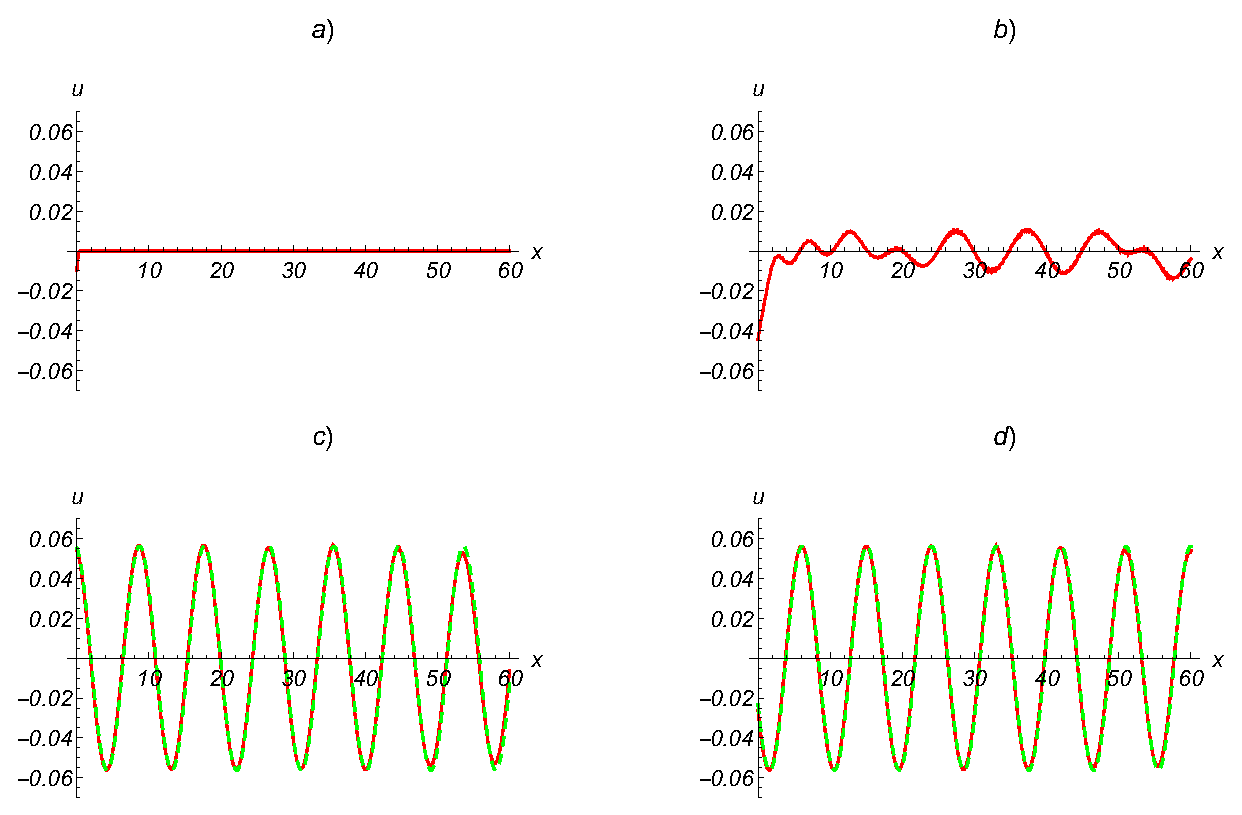
\includegraphics[width=1.0\textwidth]{new_pic/fig6.eps}
\end{center}
%\caption{Control of evolution of $u$ wave inside  the band gap, $\omega=0.35$,  when the control switches-on at $t=t_N/4$.   a)$t=0$; b)$ t=t_N/4$ ; c) $t=t_N/2$; d)$t=t_N$. Shown by dashed line in the last two stages  is the imagine part of the  exact solution (\ref{solwave}) .}
\caption{Управление эволюцией $ u $ волны внутри запрещенной зоны, $\omega=0.35$, при включении управления в момент $t=t_N/4$. a)$t=0$; b)$ t=t_N/4$; c) $t=t_N/2$; d)$t=t_N$. Пунктирной линией на последних рисунках обозначена мнимая часть точного решения (\ref{solwave}).}
\label{fg6}
 \end{figure*}
%Inside the band gap, $\sqrt{\beta_1}<\omega<\sqrt{\beta_1(1+\eta)}$,  $\omega=0.35$ there is no even a wave with decreasing amplitude. Shown in Fig.\ref{fg3} is a stromg decrease in the amplitude of disturbances and their chaotic character. This is in an agreement with the analysis from the previous Section.
Внутри запрещенной зоны $ \sqrt {\beta_1} <\omega <\sqrt {\beta_1 (1+ \eta)} $, $ \omega = 0.35 $ нет даже волны с убывающей амплитудой. На Рис. \ref{fg3} показано резкое уменьшение амплитуды возмущений и их хаотический характер. Это согласуется с анализом из предыдущего раздела.


%Further increase in the value of the excitation frequency results in the realization of the dynamics shown in Fig. \ref{fg2} when the frequency achieves the value of the upper boundary of band gap. At higher frequencies a formation of periodic wave happens with the frequency belonging to the optic branch, $\omega=\omega_o$. Again the similarity with the exact solution is observed like that shown in Fig.\ref{fg1}.
Дальнейшее увеличение значения частоты возбуждения приводит к реализации динамики, показанной на рис. \ref {fg2}, когда частота достигает значения верхней границы запрещенной зоны. На более высоких частотах происходит формирование периодической волны с частотой, принадлежащей оптической ветви, $ \omega = \omega_o $. Снова наблюдается сходство с точным решением, как показано на рис. \ref {fg1}.

  
%\section{Control of harmonic waves}
\section{Управление гармоническими волнами} 

%The use of electromegnetic signals  in \cite{Yang,Chen2014,Xiao2015} to change the internal properties of a metamaterial suggests the mechanism of a control based on an instant switch-on. It is modelled by the unit step function $H(t_0-t)$ that switches-off  the coupling in Eqs.  (\ref{eq3}), (\ref{eq4}) at$t=t_0$. Thus, for $u$ we have
Использование электромагнитных сигналов в \cite {Yang, Chen2014, Xiao2015} для изменения внутренних свойств метаматериала предполагает механизм управления, основанный на мгновенном включении. Он моделируется функцией Хэвисайда $ H (t_0-t) $, которая отключает связь в уравнениях (\ref{eq3}), (\ref{eq4}) при $ t = t_0 $. Таким образом, для $ u $ имеем
\[
u_{tt}=\beta_0 h^2 u_{xx}+\eta \beta_1 (v-u)~H(t_0-t)
\]
%Also, the unit step function should be added in equation of motion  (\ref{eq4}) and  boundary condition for $v$ (\ref{bcv}). The switch-on time for the control , $t_0$, is chosen equal to $t_N/4$, other parameters of calculations are the same as in the previous Section.
Кроме того, функция Хэвисайда должна быть добавлена в уравнение движения (\ref {eq4}) и граничное условие для $ v $, уравнение (\ref{bcv}). Время включения управления $ t_0 $ выбрано равным $ t_N / 4 $, остальные параметры вычислений выбраны такими же, как в предыдущем разделе.

%Again the comparison with the exact solution will be given.  However, after switch-on the control, equation of motion for $u$ becomes the linear wave equation whose solution is
Снова результаты расчетов будут сравниваться с точным решением в виде гармонической волны. Однако после включения управления уравнение движения для $ u $ становится линейным волновым уравнением, решение которого имеет вид
\begin{equation}\label{solwave}
u_w=\frac{\beta_1-\omega^2}{\beta_1}~B~{\text{sin}}  (\imath(\omega/a~ x - \omega~ t-\omega/a~ x_0))
\end{equation}
%Then the comparison will be done with different solutions before and after switch-on the control.
Затем будет проведено сравнение с разными решениями до и после включения управления. 
 
%Shown in Fig \ref{fg4} is the generation of the harmonic waves at $\omega=0,2$ when the control switches on at the stage b).  A comparison with the solution (\ref{solfin}) demonstrates partial similarity between the analytical and numerical solution. However, contrary to Fig. \ref{fg1}, the stages c) and d) show the tendency to the solution (\ref{solwave}) . So the control provides a transition from one harmonic wave to another.
На Рис. \ref{fg4} показана генерация гармонических волн при $ \omega = 0.2 $ при включении управления на этапе b). Сравнение с решением (\ref{solfin}) демонстрирует частичное сходство между аналитическим и численным решениями. Однако, в отличие от рис. \ref{fg1}, этапы c) и d) демонстрируют тенденцию сходимости к решению (\ref{solwave}). Таким образом, управление обеспечивает переход от одной гармонической волны к другой.

%An increase in the excitation frequency up to the lower boundary of the band gap shown in Fig. \ref{fg5} did not result in the harmonic wave without control as shown in Fig. \ref{fg2}. Here the switch-on the control at $t_0=t_N/4$ results in the formation of the harmonic wave whose shape is close to the analytical solution shown by dashed line  (\ref{solfin}).
Увеличение частоты возбуждения до нижней границы запрещенной зоны, показанной на Рис. \ref{fg5}, не привело к возникновению гармонической волны без управляющего воздействия, как показано на рис. \ref{fg2}. В этом случае включение управления при $ t_0 = t_N / 4 $ приводит к формированию гармонической волны, форма которой близка к аналитическому решению, показанному пунктирной линией (\ref {solfin}).

%The same happens for the excitation frequency $\omega=0.35$ inside the band gap. Shown in Fig. \ref{fg6} is the formation of the harmonic wave whose shape is close to the analytical solution shown by dashed line  (\ref{solfin})  contrary to the no propagation scenario shown in Fig. \ref{fg3}.
То же самое происходит с частотой возбуждения $\omega = 0.35 $ внутри запрещенной зоны. На Рис. \ref {fg6} демонстрируется формирование гармонической волны, форма которой близка к аналитическому решению, показанному пунктирной линией (\ref {solfin}), что находится в существенном отличии со сценарием, показанным на Рис. \ref {fg3}, где волна не распространяется.


%\section{Discussion}
\section{Выводы}

%The boundary excitation can generate harmonic waves in the metamaterial in an agreement with the results obtained on the basis of the particular traveling wave solution. However, the area of the values of the frequency where no periodic waves propagates turns out wider than that predicted by the analysis of the dispersion relation. Besides the band gap zone where no waves propagate, there is an interval where non-periodic waves travel.
Граничное возбуждение может генерировать гармонические волны в метаматериале, что согласуется с результатами, полученными на основе конкретного решения в виде бегущей волны. Однако область значений частоты, в которой периодические волны не распространяются, оказывается шире, чем предсказывается анализом дисперсионного соотношения. Помимо зоны запрещенной зоны, где волны не распространяются, существует интервал, в котором распространяются непериодические волны.

%The switch-on control allow us to provide harmonic waves generation inside and outside the band gap. Such mechanism of control could be realized using the experimental set-up developed in \cite{Yang}. Similar to this paper, one can not only switch- off the internal oscillator but change its properties.
Управление включением позволяет обеспечивать генерацию гармонических волн внутри запрещенной зоны и за ее пределами. Такой механизм контроля может быть реализован на экспериментальной установке, разработанной в \cite{Yang}. При этом предполагается, что можно не только выключить внутренний осциллятор, но и изменить его свойства.

%Further perspectives could be related to the active metamaterial with an external force accounting for the feedback control \cite{Pope2012,Pope2014}. In this case application of the feedback speed-gradient control  method developed in our early works \cite{bound_fradkov,  Porubov etal.2016}, looks promising. Of special interest is the inclusion of nonlinearity in the model of the metamaterial and development of the nonlinear methods of control.
Дальнейшие перспективы могут быть связаны с рассмотрением модели активного метаматериала под действием внешней силы, обеспечивающей управление обратной связью \cite{Pope2012, Pope2014}. В этом случае перспективным выглядит применение управления с обратной связью методом скоростного градиента, разработанного в работах \cite{bound_fradkov, porant16}. Особый интерес представляет учет нелинейности в модели метаматериала и развитие нелинейных методов управления.